% 3d-torus.tex
\documentclass[border=5pt]{standalone}
%%%<
\usepackage{verbatim}
%%%>
\usepackage{pgfplots}
\pgfplotsset{width=7cm,compat=1.8}

\begin{comment}
:Title: Torus
:Tags: Surface plots
:Author: cmhughes
:Slug: torus

For drawing a torus, we can parametrize the surface as (for example)

x(t,s) = (2+cos(t))*cos(s+pi/2) 
y(t,s) = (2+cos(t))*sin(s+pi/2) 
z(t,s) = sin(t)

where both t and s take values on [0,2pi].

This code was written by cmhughes on TeX.SE.
\end{comment}

\begin{document}
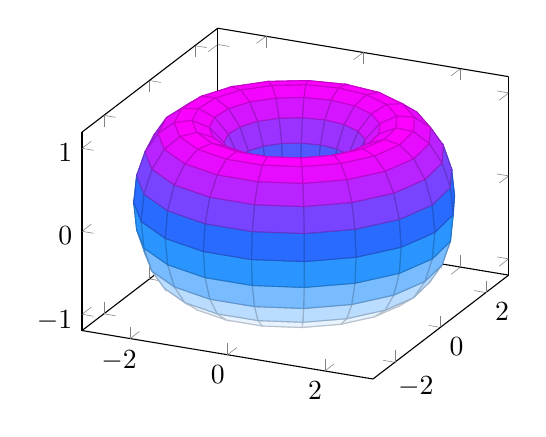
\begin{tikzpicture}
  \begin{axis}
     \addplot3[
         surf,
         colormap/cool,
         samples=20,
         domain=0:2*pi,
         y domain=0:2*pi,
         z buffer=sort
       ]
       ( {(2+cos(deg(x)))*cos(deg(y+pi/2))}, 
         {(2+cos(deg(x)))*sin(deg(y+pi/2))}, 
         {sin(deg(x))}
       );
  \end{axis}
\end{tikzpicture}
\end{document}